\documentclass[12pt]{article} %set font size and document type
\usepackage{graphicx} % Required for inserting images
\usepackage[useregional]{datetime2} %allow use of \today
\usepackage[margin=1in]{geometry} % set margins
\usepackage{setspace} % allow setting of double and single spacing
\usepackage{hyperref} % creates clickable table of contents
\usepackage{adjustbox} % allows us to rotate images, tables, etc.

% \usepackage{xcolor}
\usepackage{color, colortbl}

\usepackage{listings}
\newcommand{\lsin}[1]{\lstinline[columns=fullflexible,keepspaces=true,language=Java,basicstyle=\footnotesize\ttfamily]{#1}}

\lstdefinelanguage{Java}{
  columns=fullflexible,keepspaces=true,basicstyle=\scriptsize\ttfamily,
%  basicstyle=\scriptsize\sffamily,
  numbers=left,
  xleftmargin=5.0ex,
  escapechar=@,
  sensitive=true,
  otherkeywords={},
  morekeywords=[1]{int,while,if,public,static,else,return,new,for,return,void},
  keywordstyle={[1]\bfseries\color{blue}},
  numberstyle=\tiny\color{black},
  rulecolor=\color{black},
}

% set up header and footer
\usepackage{titleps,kantlipsum}
\newpagestyle{mypage}{%
  \headrule
  \sethead{\MakeUppercase{\thesection\quad \sectiontitle}}{}{\thesubsection\quad \subsectiontitle}
  \setfoot{}{}{\em{p. \thepage}}
}
\settitlemarks{section,subsection}
\pagestyle{mypage}

% set up title information 
% Students replace project title and their names here
\title{War Card Game
\\
CS482 Software Engineering}
\author{Ayoposi Olu-Bamisaye, Jonathan Ramos, Brett Bonner\\
Client: Dr. Eric Cui}
\date{\today}

\begin{document}

\maketitle

\pagebreak


\section{Design}

\subsection{Architecture}
We are planning on implementing a Model View Controller (MVC) architecture type for our game. It will be able to handle our in-game logic and how the user interacts with the game itself.
The Model typically will represent the game logic, deck and cards. The View will be responsible for representing the current state of the game to the user. Examples of this are displaying the players stats, profile and friends, having the ability to view output of cards/deck and showing tables in the lobby. We will be using a graphical feature to show this in our project. The Controller will handle user input for various commands like starting the game, ending the game, placing cards, party privacy and updating the players profile settings.

\subsection{Technologies}
Since we are developing a web-based version of the card game ``War", we have decided to use modern web technologies to ensure we have a responsive and scale-able application. Our front end will consist of common technologies used for web development, HTML, CSS, and Javascript. HTML will provide the basic structure of the web page, and CSS will allow us to style the page according to the theme specified by Cosmic Radiance. Javascript will handle game logic on the client side. Our front-end framework will be React.js as this will facilitate with updating the game-state without refreshing the page. React will also help with creating reusable components such as the cards themselves. 

Our back end will need to handle the game logic, player data, and real-time communication. Node.js will allow us to handle game logic outside of the browser. This will allow us the necessary means of handling requests such as determining winners. We will use a library Socket.io to handle real-time communication between multiple clients. 

To store our user data, game history, and player stats we will need persistent storage. We have chosen Firebase as our persistent storage due to its ease of use with real-time updates. It will also allow us to have a more flexible schema as SQL databases require relations among the tables created. Firebase also includes built-in authentication, supporting Google and Facebook sign in, as well as traditional email and password. Overall, Firebase supports our needs of real-time updates, scalability, security, and rapid development. 

\subsection{Persistent Storage}
Our long term data will be stored in documents. The data will be organized as JSON documents which are then organized into collections. Our users will all be stored in a collection. The collection will hold documents, and each document will hold information related to one player. Each document is the equivalent of one player and therefore, each player will need to have their own document to store their information. Another collection that we will implement is the leader-board. Each document in the leader-board collection will contain information regarding the player that has achieved recognition. This structure is flexible, making it scale-able which is important for an online multiplayer game. Our NoSQL design ensures that we can continue adding more collections and documents as needed without restructuring the entire database.

\subsection{Coding Standards}
Our database naming scheme will consist of singular, lowercase names for collections (user, leaderboard). Each attribute within documents will use camelCase (userName, gameStats, gameID). Variables and functions in JavaScript should also be written in camelCase. 

We will format our code using two spaces for indentation. Brackets should be used on the same line for functions and other control statements. Inline commenting should be used only to explain complex logic. Multi line comments should be used to describe functions and classes. Additionally, all functions should be properly documented with a multi-line comment describing the purpose, parameters, and return value. 

Testing standards will consist of test-driven development. We will ensure proper functionality by ensuring that all code commits pass necessary code tests before merging. Code tests should handle correctness, edge cases, and performance. 




\section{UML Diagram}
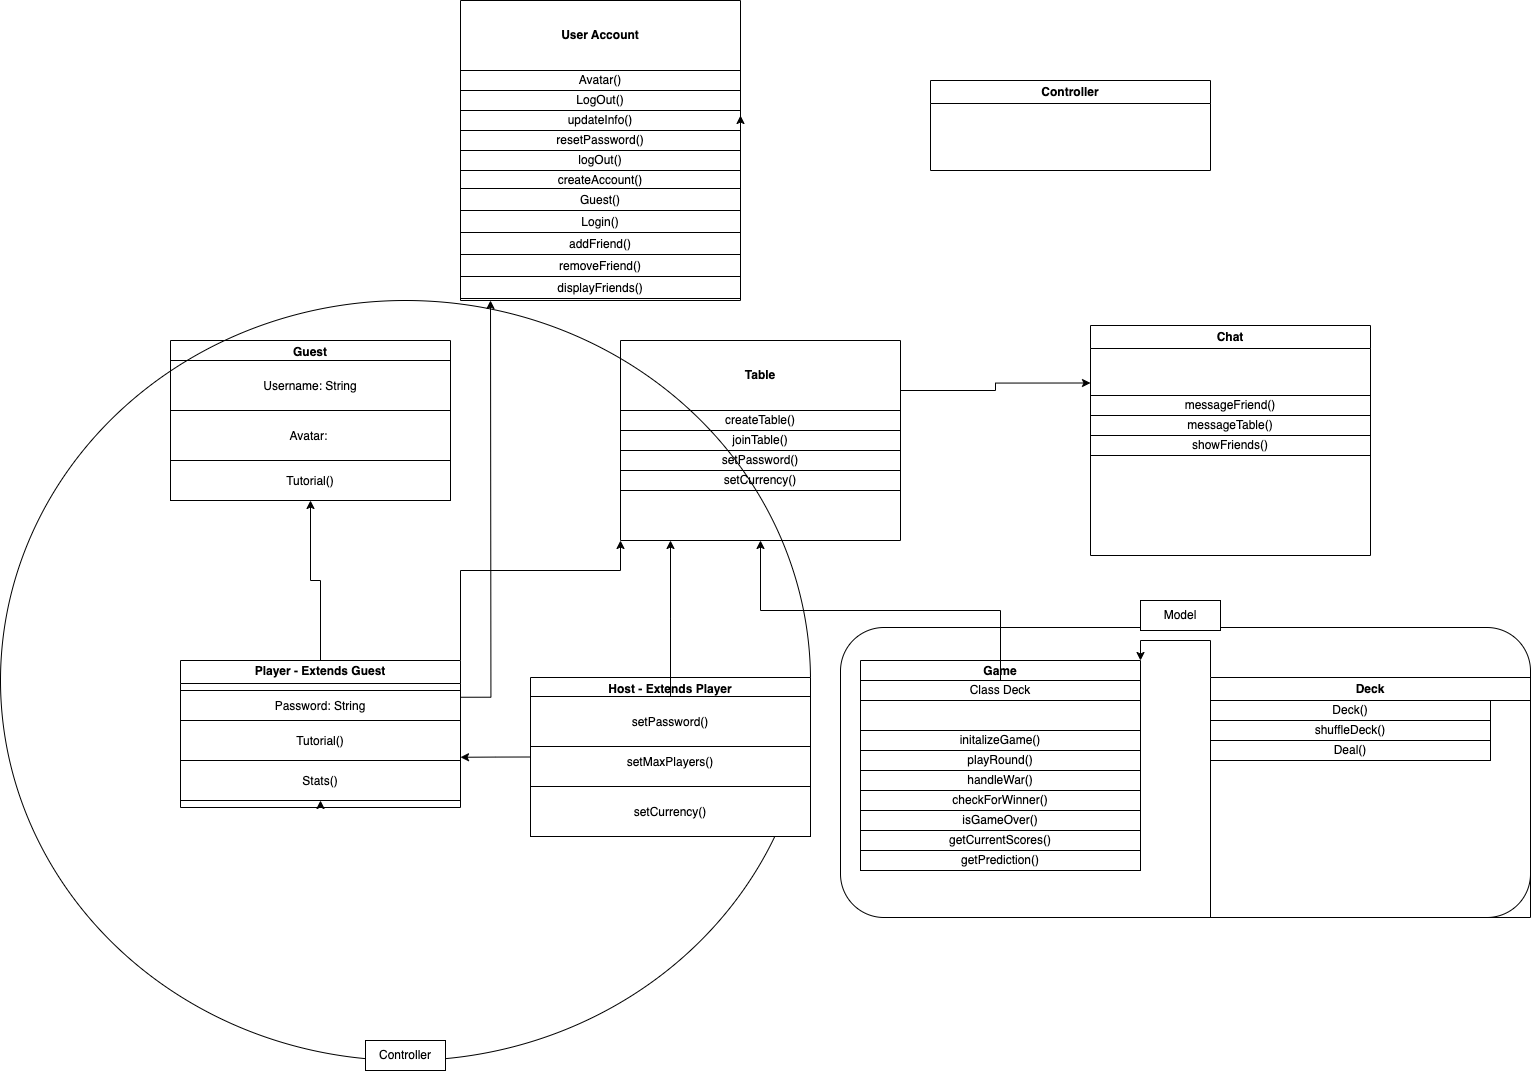
\includegraphics[width=\textwidth]{figures/WarUML.png}

The UML diagram creates an outline of the War card game for Cosmo Radiance. The system features a Host class that extends the player class, granting the host control over the table, including decisions on who can join. Additionally, a Game class manages the gameplay mechanics, ensuring that the rules of the game are followed. The User Account class manages all of the information of the User, from their password to avatar, to their friends. Lastly, a table class is made to allow users to join the table or create their own table.


\section{UI Mockups}
\includegraphics[width=\textwidth]{figures/Welcome Page UI.png}
The UI design for Cosmic Radiance web app's welcome screen features a space-themed layout with royal blue tones.

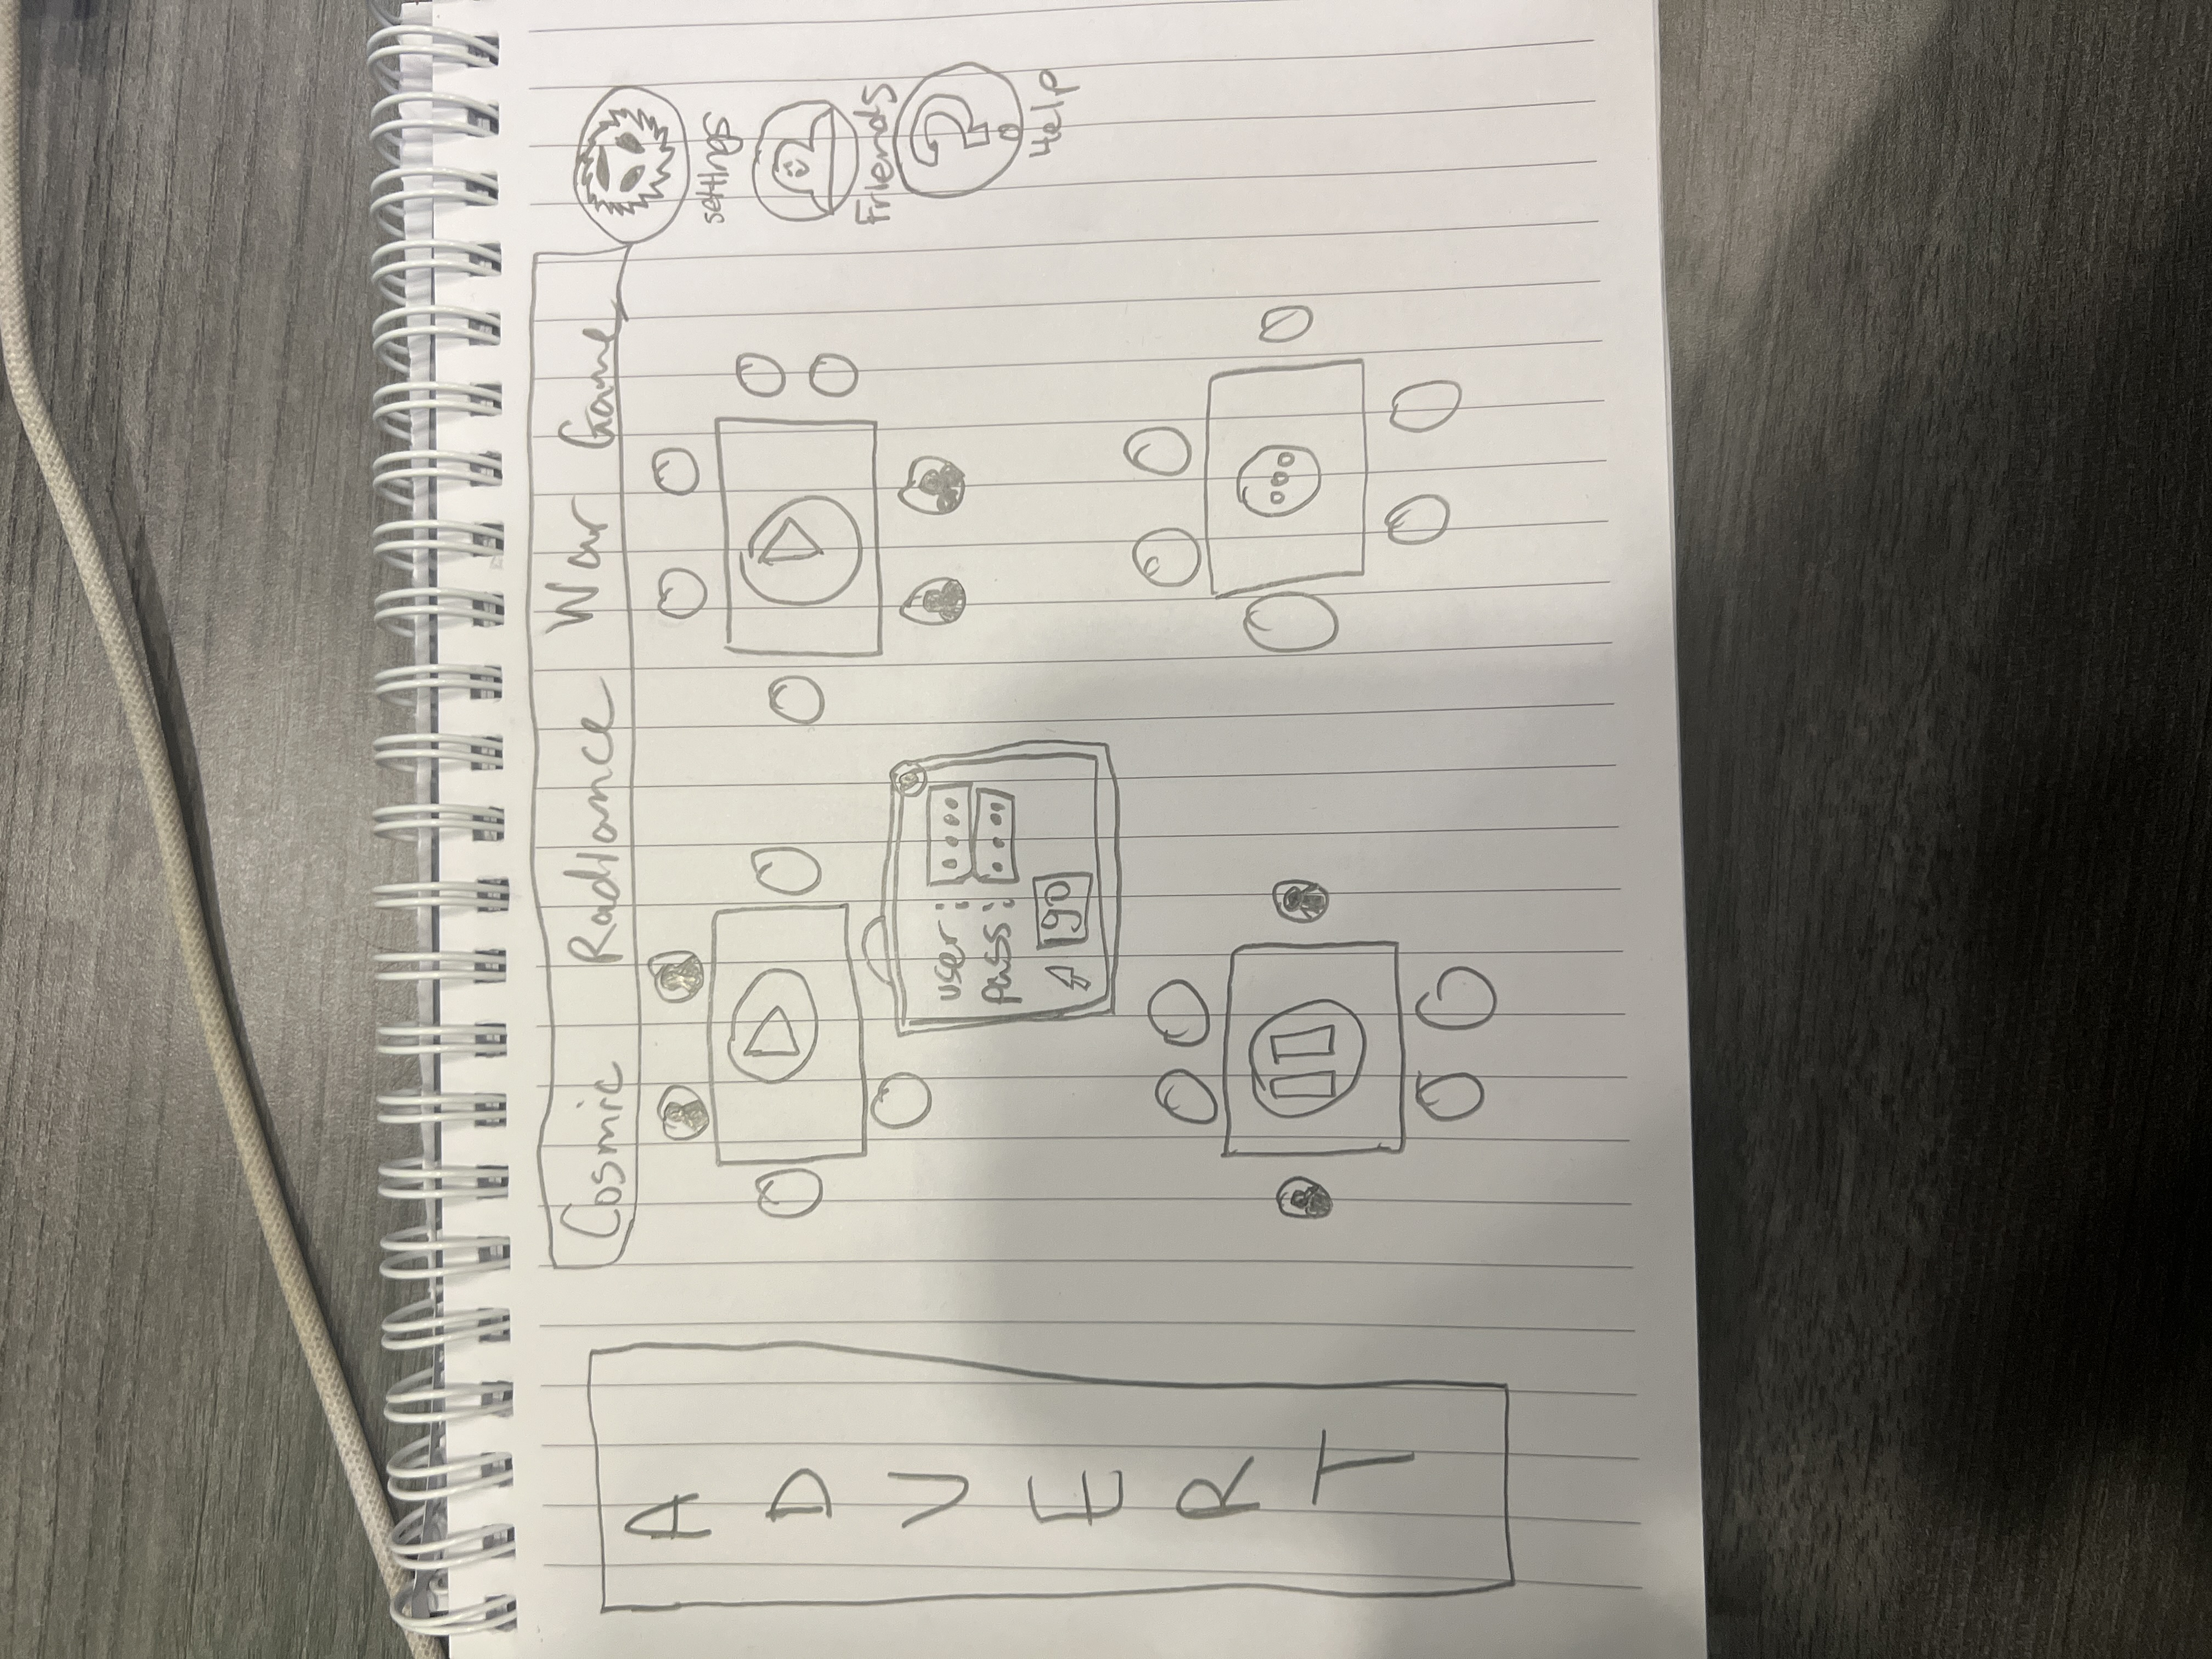
\includegraphics[width=\textwidth]{figures/Lobby UI.jpeg}

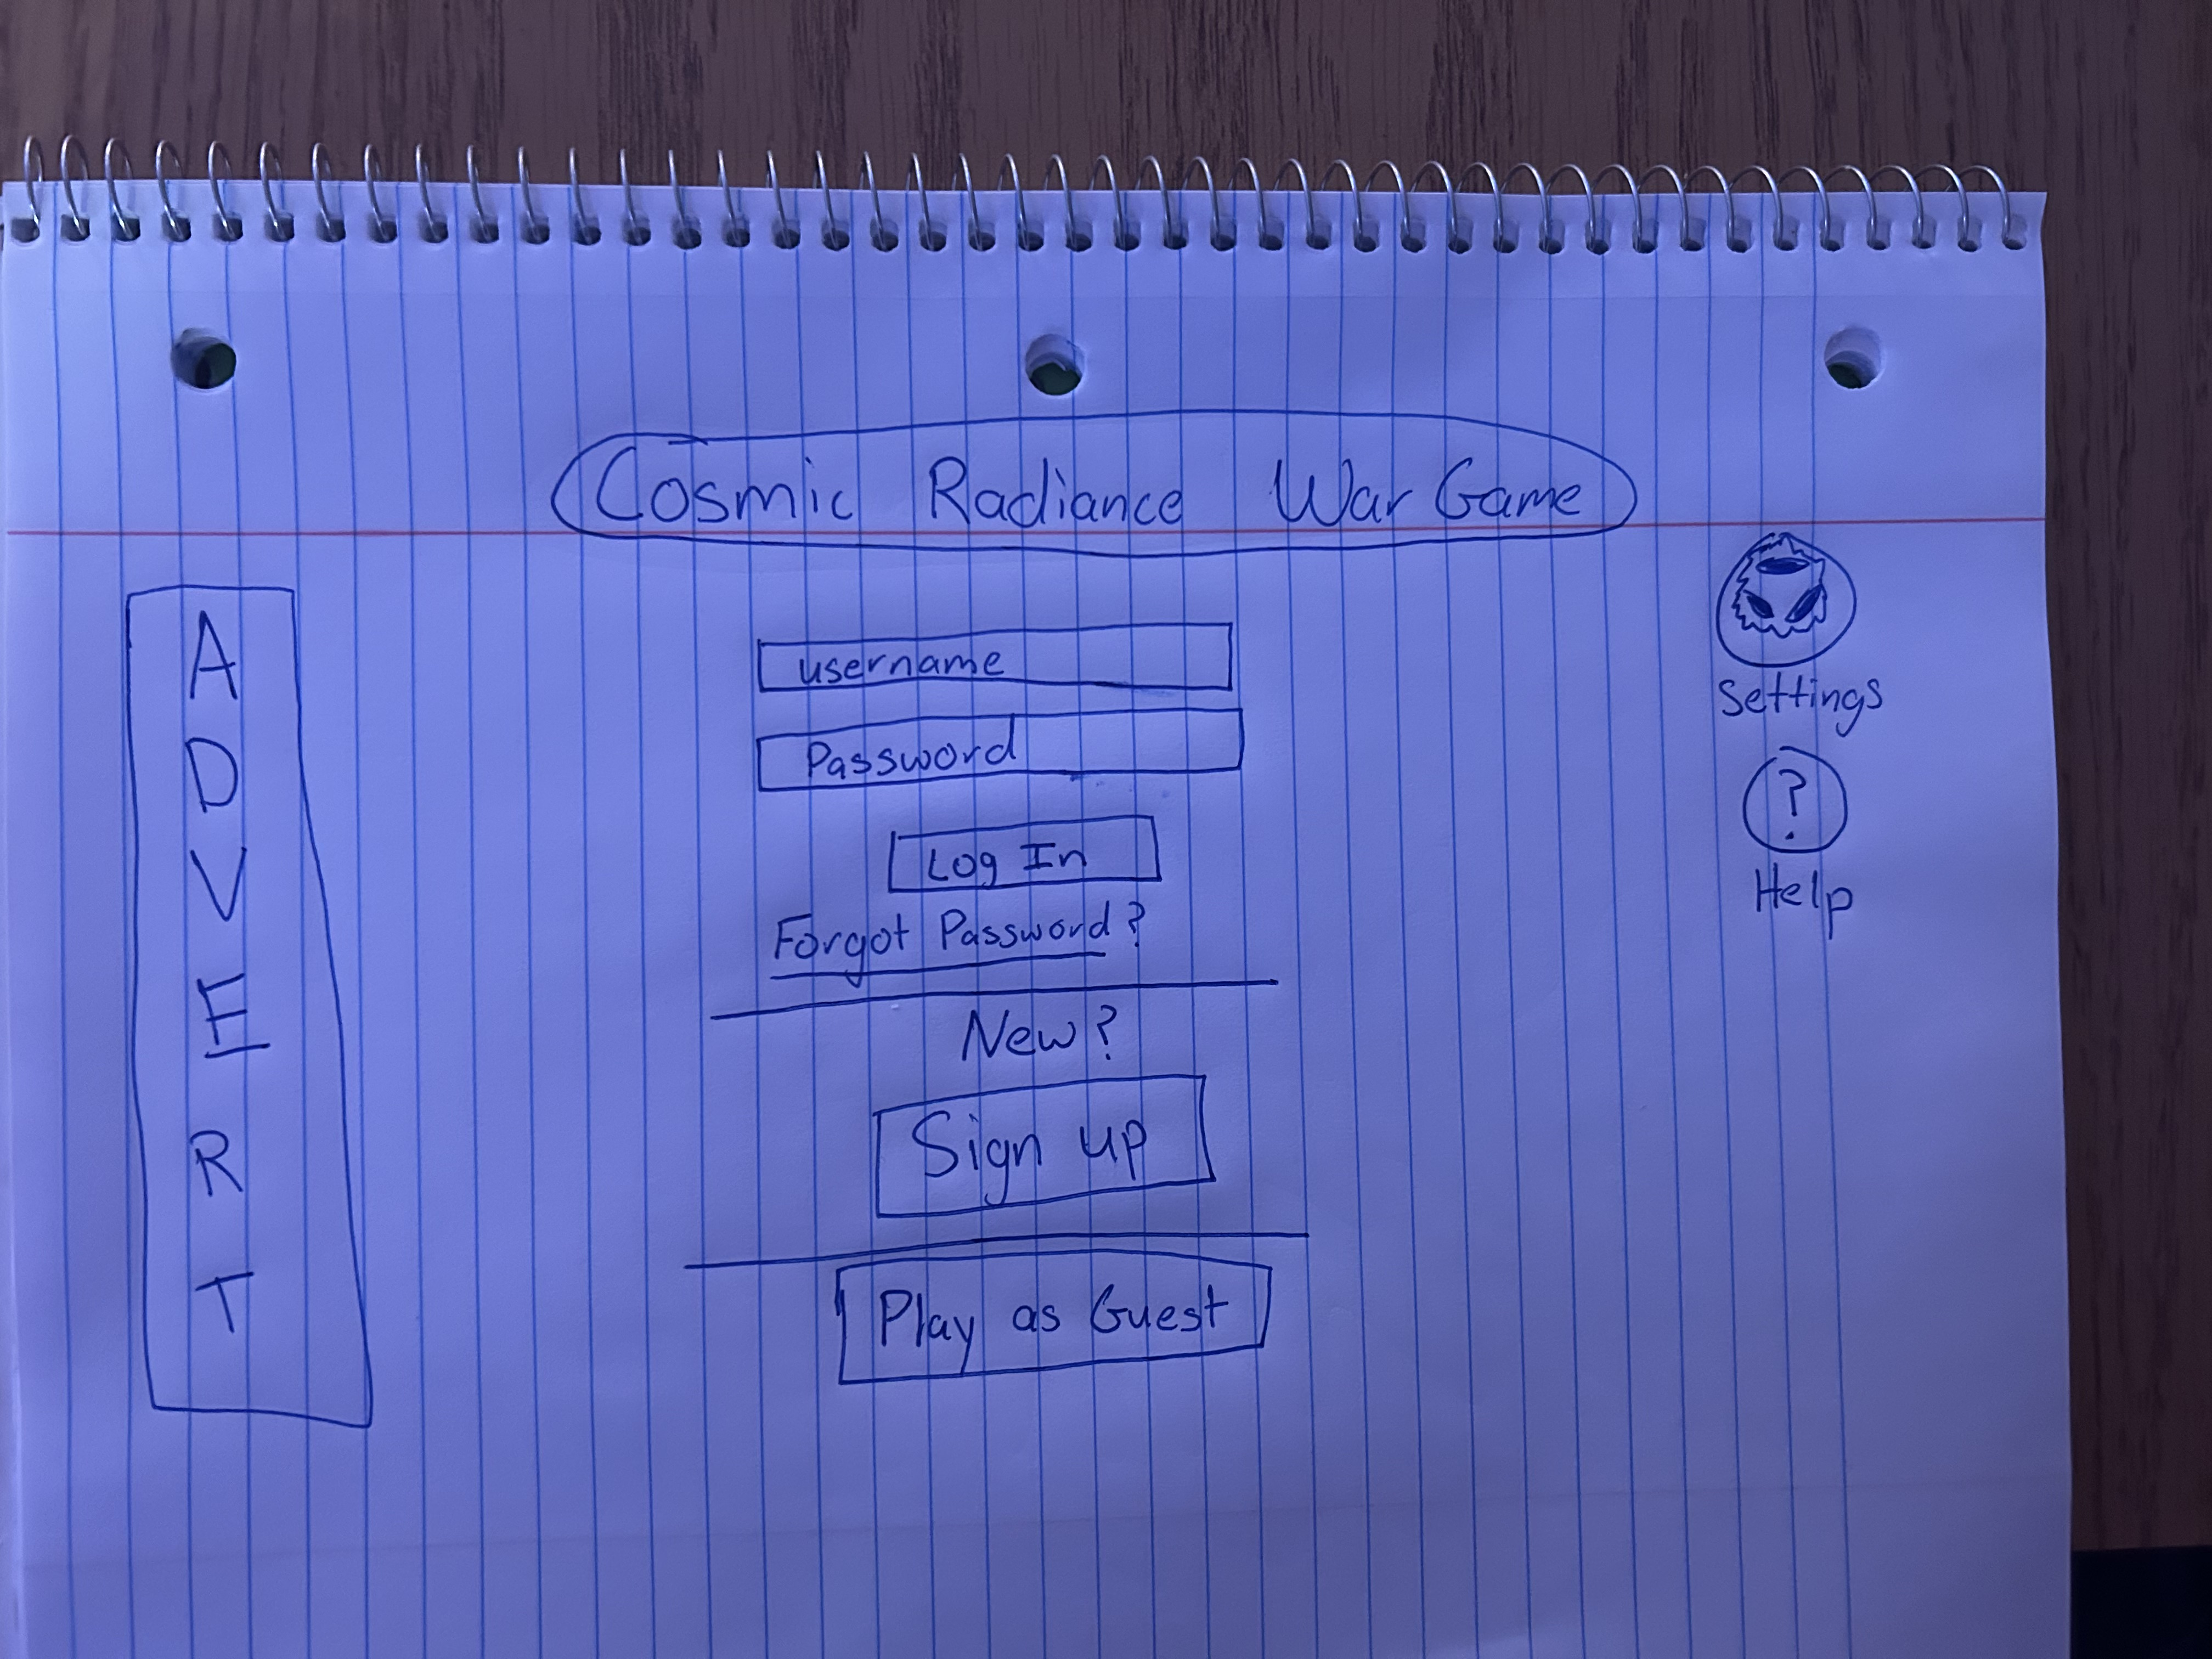
\includegraphics[width=\textwidth]{figures/Login UI.jpeg}
Login Screen for Cosmic Radiance War Game.

\end{document}

